\documentclass[conference]{IEEEtran}
\IEEEoverridecommandlockouts
% The preceding line is only needed to identify funding in the first footnote. If that is unneeded, please comment it out.
\usepackage{cite}
\usepackage{amsmath,amssymb,amsfonts}
\usepackage{algorithmic}
\usepackage{graphicx}
\usepackage{textcomp}
\usepackage[pdftex,dvipsnames]{xcolor}
\setlength {\marginparwidth }{2cm}
\usepackage[colorinlistoftodos,prependcaption,textsize=tiny]{todonotes}
\def\BibTeX{{\rm B\kern-.05em{\sc i\kern-.025em b}\kern-.08em
    T\kern-.1667em\lower.7ex\hbox{E}\kern-.125emX}}
\begin{document}
\documentclass[main.tex]{subfiles}

\begin{document}


\begin{abstract}
Se ecualizó una señal en un enlace digital basándose en el 
esquema de filtrado de inversión de sistemas. Se implementó
NLMS, justificando la elección de los parámetros, consiguiendo
minimizar el bit error rate, la tasa de errores. Luego se buscó de manera exitosa 
implementar RLS, consiguiendo aún mejores resultados para el problema.
\end{abstract}


\section{Introducción}
Se buscó ecualizar una señal en un enlace digital de comunicaciones. 
Los datos consistían en una secuencia de datos pseudoaleatoria 
codificada por Manchester, muestreada a una frecuencia de sampleo
 de 4 kHz a razón de 250 bps. Ante estas características, cada bit consiste de 
 16 muestras según la codificación mencionada. El canal, en este caso, conocido, 
 modificaba la señal dependiendo del posicionamiento
 aleatorio de dos pares de polos conjugados. En lo que respecta a estacionaridad, 
 el canal carece de la misma debido a sus características cambiantes en el tiempo.
La principal dificultad consistía entonces en la variabilidad del canal. En las 
siguientes figuras se puede notar el efecto de lo mencionado, siendo la 
señal en azul los bits enviados y en naranja lo recibido. \newline

\begin{figure}[H]
    \centering
    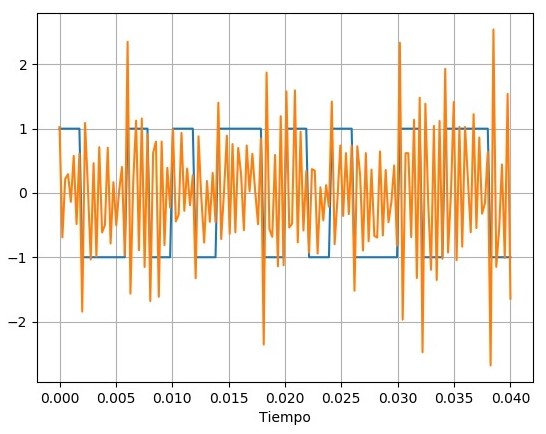
\includegraphics[scale=0.5]{imagenes/1.jpeg}
\end{figure}
\begin{figure}[H]
    \centering
    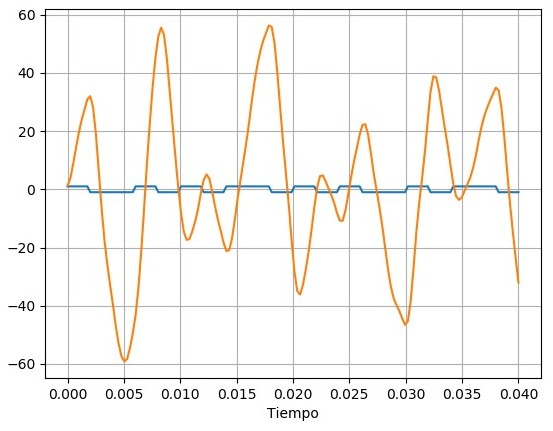
\includegraphics[scale=0.5]{imagenes/2.jpeg}
\end{figure}
\begin{figure}[H]
    \centering
    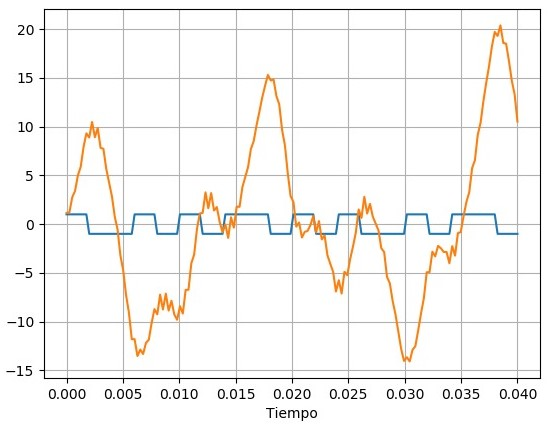
\includegraphics[scale=0.5]{imagenes/3.jpeg}\\
    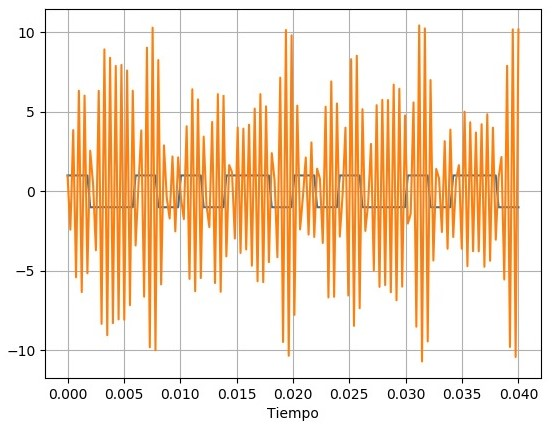
\includegraphics[scale=0.5]{imagenes/4.jpeg}
    \caption{Señales obtenidas en el receptor, al pasar por el canal.}
\end{figure}

El proyecto consiste en aplicar un algoritmo de filtrado adaptativo
 para recuperar la señal transmitida asumiendo que no se conoce la entrada, 
 lo que simularía un enlace digital de comunicaciones.
 Un esquema de lo mencionado
se puede ver en la siguiente figura.

\begin{figure}[H]
    \centering
    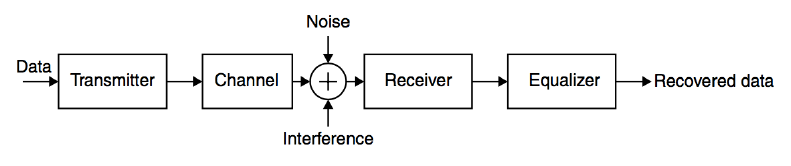
\includegraphics[scale=0.5]{imagenes/preblock.png}
    \caption{Esquema del enlace digital.}
\end{figure}

Como criterio de validación del algoritmo como así de sus parámetros, se calculó el bit error rate (BER), la
cantidad de bits errados por unidad de tiempo.



\end{document}


\section{Filtrado Adaptativo por Inversión de Sistemas}


\section{Análisis del Canal}

\section{Filtro Adaptativo}
por que no otros
\subsection{LMS}
\subsection{NLMS}

\section*{Acknowledgment}

The preferred spelling of the word ``acknowledgment'' in America is without 
an ``e'' after the ``g''. Avoid the stilted expression ``one of us (R. B. 
G.) thanks $\ldots$''. Instead, try ``R. B. G. thanks$\ldots$''. Put sponsor 
acknowledgments in the unnumbered footnote on the first page.

\section*{References}

Number footnotes separately in superscripts. Place the actual footnote at 
the bottom of the column in which it was cited. Do not put footnotes in the 
abstract or reference list. Use letters for table footnotes.


\begin{thebibliography}{00}
\bibitem{b1} G. Eason, B. Noble, and I. N. Sneddon, ``On certain integrals of Lipschitz-Hankel type involving products of Bessel functions,'' Phil. Trans. Roy. Soc. London, vol. A247, pp. 529--551, April 1955.
\bibitem{b2} J. Clerk Maxwell, A Treatise on Electricity and Magnetism, 3rd ed., vol. 2. Oxford: Clarendon, 1892, pp.68--73.
\bibitem{b3} I. S. Jacobs and C. P. Bean, ``Fine particles, thin films and exchange anisotropy,'' in Magnetism, vol. III, G. T. Rado and H. Suhl, Eds. New York: Academic, 1963, pp. 271--350.
\bibitem{b4} K. Elissa, ``Title of paper if known,'' unpublished.
\bibitem{b5} R. Nicole, ``Title of paper with only first word capitalized,'' J. Name Stand. Abbrev., in press.
\bibitem{b6} Y. Yorozu, M. Hirano, K. Oka, and Y. Tagawa, ``Electron spectroscopy studies on magneto-optical media and plastic substrate interface,'' IEEE Transl. J. Magn. Japan, vol. 2, pp. 740--741, August 1987 [Digests 9th Annual Conf. Magnetics Japan, p. 301, 1982].
\bibitem{b7} M. Young, The Technical Writer's Handbook. Mill Valley, CA: University Science, 1989.
\end{thebibliography}
\vspace{12pt}
\color{red}
IEEE conference templates contain guidance text for composing and formatting conference papers. Please ensure that all template text is removed from your conference paper prior to submission to the conference. Failure to remove the template text from your paper may result in your paper not being published.

\end{document}
